\documentclass[11pt]{paper}

\usepackage[T1]{fontenc}

\usepackage{graphicx}
\usepackage{amssymb}
\usepackage{amstext}
\usepackage{amsmath}
\usepackage{a4wide,color}
\usepackage[utf8]{inputenc}
\usepackage[frenchb]{babel}
\usepackage{xspace}
\usepackage{anysize}
\usepackage{tabularx}
\usepackage{multirow}
\usepackage{fancybox}
\usepackage{fancyhdr}
\usepackage{bbding}

\usepackage{caption}
\usepackage{subcaption}


\usepackage{color}
\usepackage{float}

\usepackage[toc,page]{appendix} 
\usepackage{lscape}

\usepackage{placeins}

\usepackage{listings}
\lstdefinestyle{customc}{
  belowcaptionskip=1\baselineskip,
  breaklines=true,
  frame=L,
  xleftmargin=\parindent,
  language=C,
  showstringspaces=false,
  basicstyle=\tiny\ttfamily,
  keywordstyle=\bfseries\color{green!40!black},
  commentstyle=\itshape\color{purple!40!black},
  identifierstyle=\color{blue},
  stringstyle=\color{orange},
  tabsize=2
}

\usepackage{todonotes}

\usepackage[framemethod=TikZ]{mdframed}

\lstset{% general command to set parameter(s)
	basicstyle=\footnotesize, % print whole listing small
	keywordstyle=\color{magenta}\bfseries, % underlined bold black keywords
	identifierstyle=, % nothing happens
	commentstyle=\color{black}, % white comments
	stringstyle=\ttfamily, % typewriter type for strings
	showstringspaces=false % no special string spaces
} 

\lstdefinelanguage{aald}
	{morekeywords={system, implementation},
	sensitive=false,
	morecomment=[l]{//},
	morecomment=[s]{/*}{*/},
	morestring=[b]",
}

\usepackage[colorlinks=true]{hyperref}

\usepackage[normalem]{ulem}
\usepackage{color}

\definecolor{Fond}{gray}{0.7}

\renewcommand{\floatpagefraction}{.99}
\renewcommand{\textfraction}{.01}
\newcommand{\modif}[1]{\textcolor{red}{\uline{#1}}}


\pagestyle{fancy}
\fancyhf{}
\fancyhead[RE,RO]{\thepage}
\fancyhead[LE]{}
\fancyhead[LO]{Temps réel }
\fancyfoot[LO]{Centrale Nantes -- \today}
\fancypagestyle{plain}{%
  \fancyhf{} % get rid of headers
  \renewcommand{\headrulewidth}{0pt} % and the line
}

\newenvironment{maliste}%
{ \begin{list}%
	{\ArrowBoldRightStrobe}%
	{\setlength{\labelwidth}{30pt}%
	 \setlength{\leftmargin}{35pt}%
	 \setlength{\itemsep}{\parsep}}}%
{ \end{list} }

 \setlength{\parskip}{1.2ex plus .9ex minus .4ex}

\newcommand{\ocv}{{\tt OpenCV}\xspace} 
\newcommand{\alsa}{{\tt ALSA}\xspace} 
\newcommand{\aadl}{{\tt AADL}\xspace} 
\newcommand{\xeno}{{\tt Xenomai}\xspace} 
\newcommand{\iic}{I$^2$C\xspace} 


\title{{\Large Systèmes interconnectés -- SINT }\\
\vspace{-0.4em}
{\large Sujet de TP 5 : CAN et FPGA}\\
{\small Centrale Nantes}\\
\small P.-E. Hladik, \small{\texttt{pehladik@ec-nantes.fr}}\\
---\\
{\scriptsize  Version bêta (\today)}\\
}


\begin{document}

\maketitle

%\begin{table}[htdp]
%\caption{Suivi des modifications}
%\begin{center}
%\begin{tabular}{|c|c|c|p{8cm}|}
%\hline
%Date & Version & Auteur & Modifications\\
%\hline
%JJ/MM/12 & 0.3.X & P.-E. Hladik&  \\
%\hline
%\end{tabular}
%\end{center}
%\label{default}
%\end{table}%

%%%%%%%%%%%%%%%%%%%%%%%%%
  \section{Objectifs pédagogiques}
%%%%%%%%%%%%%%%%%%%%%%%%%


\begin{itemize}
	\item spécifier une machine séquentielle à l'aide d'un automate
	\item simuler et tester une implémentation en VHDL
	\item intégrer plusieurs entités dans un projet
	\item comprendre le calcul du CRC
\end{itemize}

%%%%%%%%%%%%%%%%%%%%%%%%%
  \section{Rendu}
%%%%%%%%%%%%%%%%%%%%%%%%%

À la fin du TP déposez sur Hippocampus une archive avec un compte rendu en pdf (voir les éléments demandés dans le texte).

%%%%%%%%%%%%%%%%%%%%%%%%%
  \section{Prise en main}
%%%%%%%%%%%%%%%%%%%%%%%%%

Cette première partie a pour but de reprendre en main Vivado et le VHDL.

\subsection{Création d'un projet}

Commencez par créer un nouveau projet sous Vivado (voir le \href{https://hippocampus.ec-nantes.fr/pluginfile.php/76485/mod_resource/content/4/TUTO%20VIVADO.pdf}{document en ligne} ou la vidéo). 
Pour cette première étape vous aurez besoin des fichiers {\tt clock\_div.vhd} %et  {\tt display\_basys3.vhd}
en tant que {\it Design Sources}, de {\tt testbench\_div.vhd} comme {\it Simulation Sources} et {\tt basys3.xdc} comme contraintes. Ces fichiers sont dans l'archive sur Hippocampus. Vous pouvez importer les fichiers à la création du projet ou bien après.

Pour la carte Basys3, il faut sélectionner le composant \og xc7a35tcpg236-1 \fg que l'on peut trouver avec le filtre :
\begin{itemize}
	\item Family : Artix-7
	\item Package : cpg236
	\item Speed : -1
\end{itemize}


\subsection{Simulation}

Vérifiez que vous avec bien importez {\tt testbench\_div.vhd} dans {\it Simulation Sources} et qu'il est bien au {\it top level} (sinon clic droit et {\it Set as Top}). Ce fichier simule le comportement d'une entité de type {\tt clock\_div}.

Lancez la simulation comportementale (voir vidéo) et observez. Pour l'instant seul le signal reset est simulé. Ajoutez le code nécessaire pour simuler l'horloge à une période de 10~ns et lancez la simulation.


\todo[inline, color=green!40]{{\bf Rapport :} mettez l'extrait de code du testbench ainsi qu'une capture de la simulation.}

Quel est le rapport cyclique si le diviseur est impair (3 par exemple) ? Observez en simulation le comportement et expliquez les raison en allant lire le code de {\tt clock\_div.vhd}.

\todo[inline, color=green!40]{{\bf Rapport :} mettez une capture de la simulation avec un diviseur de 3 et expliquez le comportement observé à partir du code.}

\subsection{Synthèse}

Assurez-vous que vous avez bien importé {\tt display\_sint.vhd} comme {\it Design Sources} et {\tt basys3.xdc} comme contraintes.

Créez un nouveau fichier de conception et mettez le comme {\it Top Level}. Implémentez un système qui fait clignoter une led toutes les 500~ms. Pour cela utilisez le diviseur d'horloge sachant que l'horloge du système a une période de 10~ns. Les signaux physiques dont vous aurez besoin sont :
\begin{itemize}
	\item {\tt led0} en sortie,
	\item {\tt reset} en entrée,
	\item {\tt clock\_100Mhz} en entrée.
\end{itemize}
\bigskip

Ils doivent être déclarés comme ports de votre entité comme dans l'exemple ci-dessous :
\begin{lstlisting}[language=VHDL]
entity blink is
  Port (
        reset 		: in std_logic;
        clock_100Mhz 	: in std_logic;
        led0 		: out std_logic
        );
end blink;
\end{lstlisting}
et seront ensuite liés aux signaux physiques dans le fichiers de contraintes (vérifiez que les lignes nécessaires dans le fichiers de contraintes {\tt basys.xdc} sont bien décommentées).

Ecrivez le code, faites la synthèse et exécutez le résultat sur la carte.

\todo[inline, color=green!40]{{\bf Rapport :} mettez le code produit.}

%%%%%%%%%%%%%%%%%%%%%%%%%
  \section{Affichage}
%%%%%%%%%%%%%%%%%%%%%%%%%

Importez dans votre projet le fichier {\tt display\_sint.vhd}.

L'entitée {\tt display\_basys3} permet d'afficher une valeur en hexadécimale sur l'afficheur 7 segments de la carte. Les ports sont :
\begin{itemize}
	\item  {\tt clock\_100Mhz} (entrée) : l'horloge physique de la carte,     %: in std_logic;-- 100Mhz clock on Basys 3 FPGA board
	\item  {\tt reset } (entrée) : le signal physique de reset de la carte,           %: in std_logic; -- reset
	\item  {\tt anode\_activate} (entrée) : les signaux physiques des anodes,   % : out std_logic_vector (3 downto 0);-- 4 Anode signals
	\item  {\tt led\_out} (entrée)  : les signaux physiques des leds de l'afficheur,        % : out std_logic_vector (6 downto 0);-- Cathode patterns of 7-segment display
	\item  {\tt displayed\_number} (entrée) : la valeur à afficher.%: in std_logic_vector (15 downto 0) -- Decimal number to be displayed on 4-digit 7-segment display
\end{itemize}

Créez un nouveau fichier et implanter un code qui met à jour toutes les secondes l'afficheur en incrémentant une valeur (vous aurez une horloge hexadécimale). Servez-vous de ce que vous avez fait avant pour le compteur en le copiant dans le nouveau fichier (ou utilisez ce que vous avez fait avant).

Si vous passez par un entier pour coder la valeur à afficher, vous pouvez utiliser

{\tt n <= std\_logic\_vector( to\_unsigned(val, n'length))} 

pour convertir l'entier non signé {\tt val} et l'affecte à un signal {\tt n} de type {\tt std\_logic\_vector} de taille {\tt n'length}.

Pour les contraintes, voir les commentaires dans le fichier {\tt display\_sint.vhd} et décommentez les lignes dans le fichier de contraintes.

\todo[inline, color=green!40]{{\bf Rapport :} mettez le code produit.}

%%%%%%%%%%%%%%%%%%%%%%%%%
  \section{Capteur ultrason}
%%%%%%%%%%%%%%%%%%%%%%%%%

Dans cette partie vous allez coder le contrôleur d'un capteur \href{https://wiki.seeedstudio.com/Grove-Ultrasonic_Ranger/}{Ultrasonic Ranger V2.0} de Grove. Le principe de fonctionnement d'un capteur à ultrason consiste à émettre
\og à intervalles réguliers de courtes impulsions sonores à haute fréquence. Ces impulsions se propagent dans l’air à la vitesse du son. Lorsqu’elles rencontrent un objet, elles se réfléchissent et reviennent sous forme d’écho au capteur. [Le capteur] calcule alors la distance le séparant de la cible sur la base du temps écoulé entre l’émission du signal et la réception de l’écho. \fg [\href{https://www.microsonic.de/fr/support/capteurs-à-ultrasons/principe.htm}{microsonic}].


Les entrées/sorties de l'ultrasonic ranger sont décrites par la figure~\ref{fig:pinout}. Le seul signal qui nous intéresse est celui identifié comme {\tt SIG}. Physiquement vous pouvez connecter le capteur sur les broches des pmod de la basys3 (voir figure~\ref{fig:pmod}).

\begin{figure}[htbp]
\begin{center}
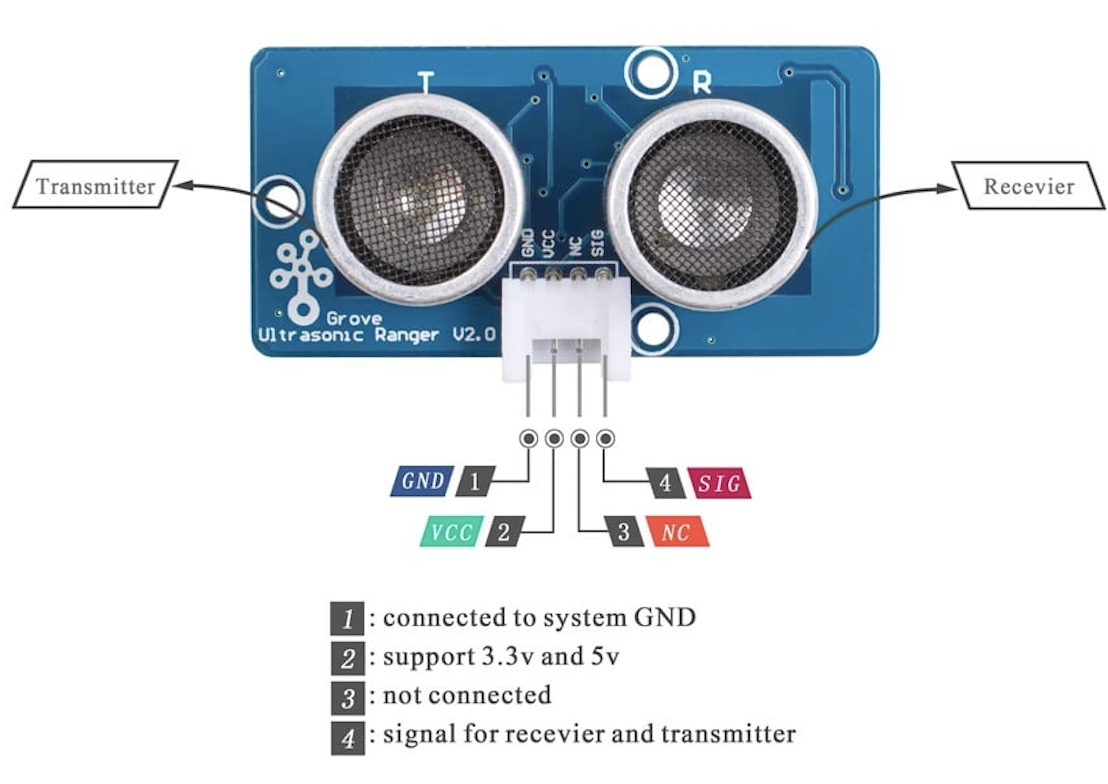
\includegraphics[scale=0.4]{./figures-pdf/pinout}
\caption{Entrée/sortie de l'Ultrasonic Ranger V2.0}
\label{fig:pinout}
\end{center}
\end{figure}

\begin{figure}[htbp]
\begin{center}
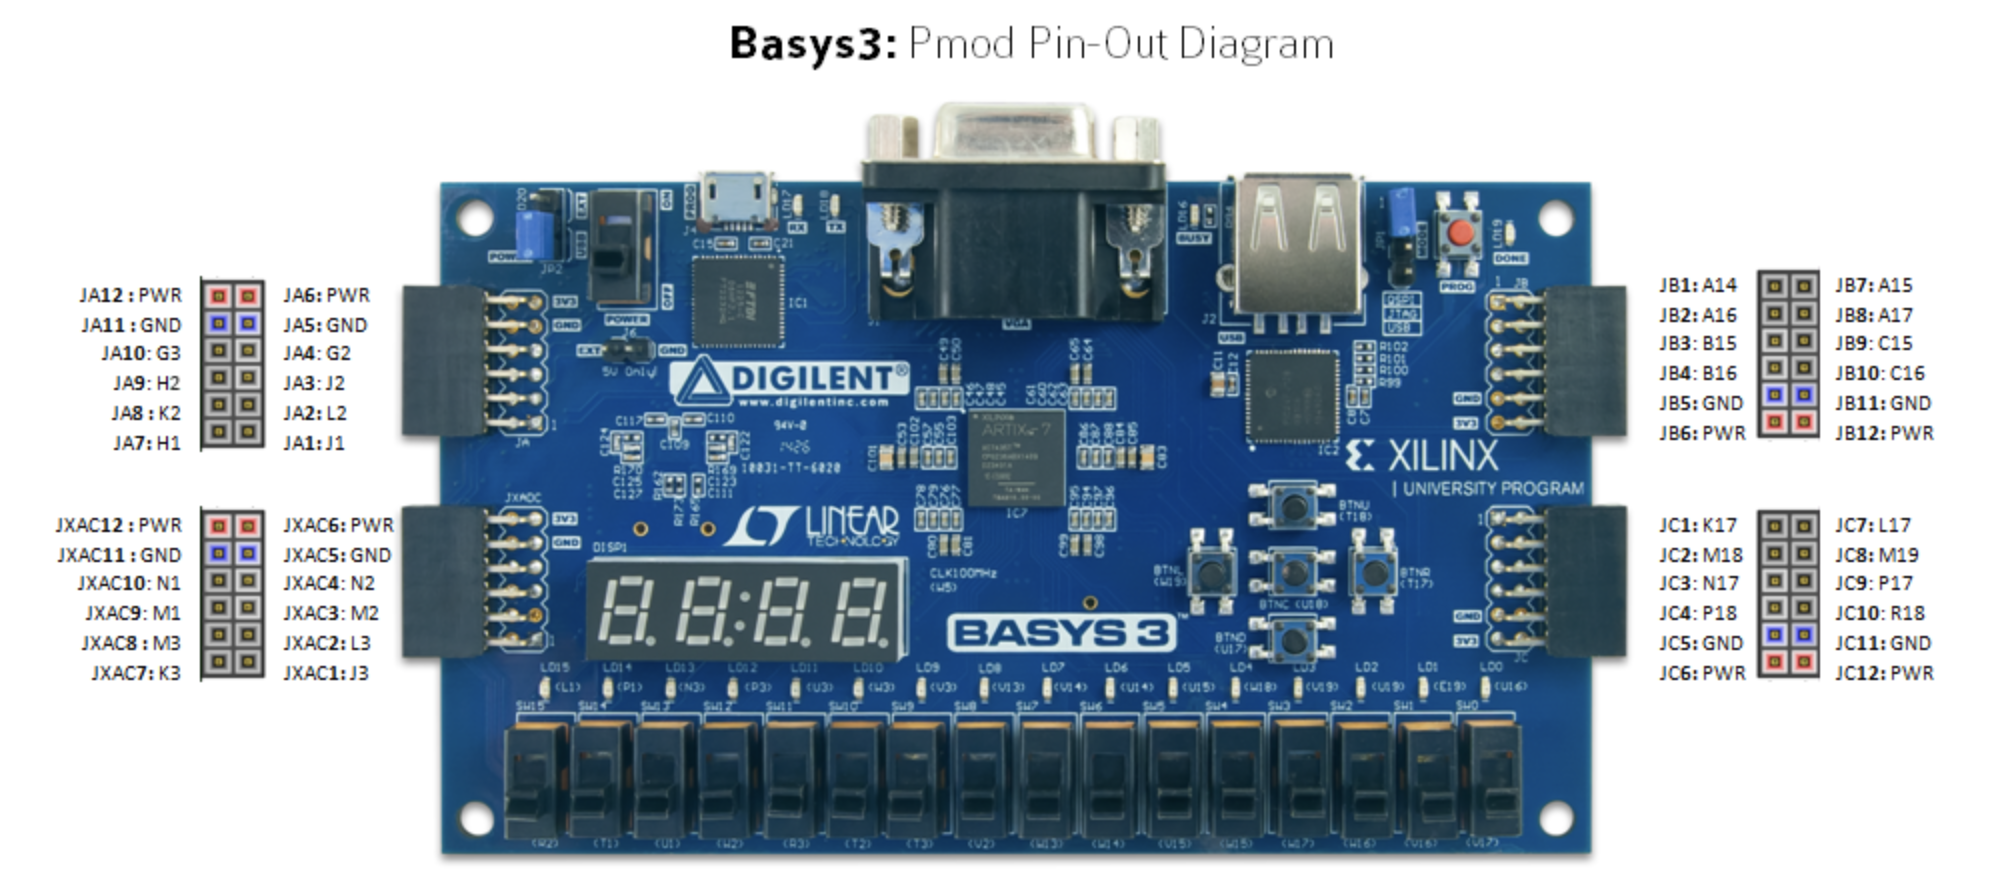
\includegraphics[scale=0.45]{./figures-pdf/pmod}
\caption{Nom des broches des pmod de la basys3}
\label{fig:pmod}
\end{center}
\end{figure}

\subsection{Spécifications}

L'entité permettant de contrôler le capteur à ultrason aura pour interface les ports suivants (voir figure~\ref{fig:port_us}) :

\begin{itemize}
\item en entrée :
\begin{itemize}
	\item clk: une horloge,
	\item rst : un signal de reset,
	\item start : un signal pour démarrer une acquisition.
\end{itemize}
\item en sortie :
\begin{itemize}
    	\item ready : un signal indiquant que le capteur est disponible pour une mesure,
	\item resReady : un signal indiquant qu'une nouvelle valeur a été produite,
	\item res : un entier avec la distance mesurée en cm,
	\item err1 : un signal en cas d'erreur de type 1 (voir après),
    	\item err2 : un signal en cas d'erreur de type 2 (voir après).
\end{itemize}
\item en entrée/sortie (inout en VHDL) :
\begin{itemize}
    	\item sig : le signal de contrôle et de donnée vers le capteur externe.
\end{itemize}
\end{itemize}

\begin{figure}[htbp]
\begin{center}
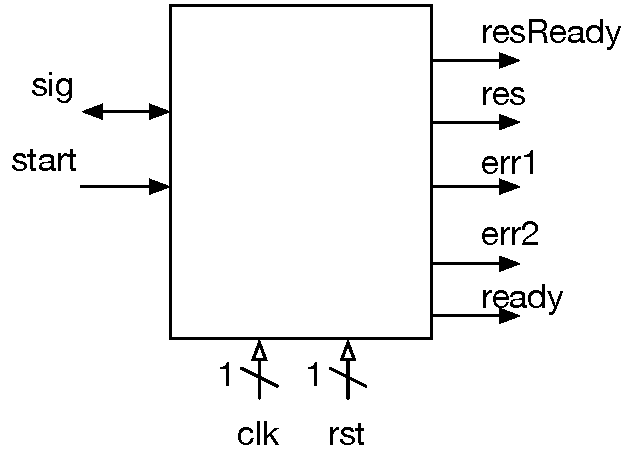
\includegraphics[scale=0.45]{./figures-pdf/port_ultrasound}
\caption{Port de l'entité ultrason}
\label{fig:port_us}
\end{center}
\end{figure}

L'entité aura aussi deux valeurs de configuration {\tt timeout1} et {\tt timeout2}.

Le fonctionnement du capteur est simple. Pour lancer une mesure, il faut maintenir sur {\tt sig} un signal à l'état haut pendant 10~$\mu$s, puis attendre de nouveau le passage à l'état haut du signal pour commencer la mesure et arrêter la mesure quand le signal repasse à l'état bas (voir figure~\ref{fig:signal}). La distance à l'obstacle est proportionelle à la durée de l'impulsion mesurée.

\begin{figure}[htbp]
\begin{center}
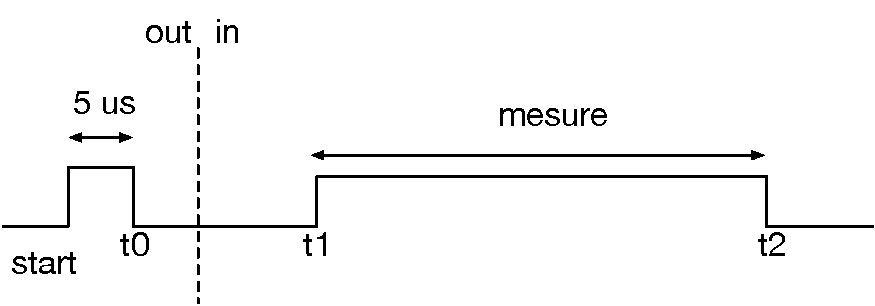
\includegraphics[scale=0.45]{./figures-pdf/signal}
\caption{Signal de contrôle et de mesure du capteur}
\label{fig:signal}
\end{center}
\end{figure}

Le contrôle à réaliser est donc le suivant :
\begin{itemize}
	\item Le signal {\tt ready} est à 1 quand le capteur est au repos et 0 sinon.
	\item Quand le signal {\tt start} est à 1 et que {\tt ready} est à 1, une impulsion de 10~$\mu$s est produite, puis le signal est placé dans l'état Z pour permettre la mesure. 
	\item La mesure est le temps de l'impulsion. Pour une impulsion $dt$ en $\mu$s, la distance est de $dt / 29 /2$ cm.
	\item Quand une mesure est produite, {\tt resReady} est mis à 1 et le résultat (en cm) est écrit dans {\tt res}.
	\item Si le temps entre {\tt t0} et {\tt t1} est supérieur à {\tt timeout1} alors une erreur de type 1 est produite (le signal {\tt err1} passe à 1).	
	\item Si le temps entre {\tt t1} et {\tt t2} est supérieur à {\tt timeout2} alors une erreur de type 2 est produite (le signal {\tt err2} passe à 1).
	\item les signaux de sortie sont tous à zéro au début et au lancement d'une nouvelle mesure.
\end{itemize}
\bigskip

Représentez la spécification du contrôleur ultrason sous forme d'un automate (Mealy ou Moore au choix).

\todo[inline, color=green!40]{{\bf Rapport :} mettre l'automate qui décrit la spécification du contrôleur ultrason.}

\subsection{Implantation}

Produisez le code de votre contrôleur ultrason.

\todo[inline, color=green!40]{{\bf Rapport :} mettre le code du contrôleur ultrason.}

\subsection{Simulation}

Faites une simulation de votre contrôleur. Pour cela vous aurez besoin de produire un signal d'horloge, mais aussi de {\tt sig} (tant que le signal est contrôlé il faut qu'il soit dans l'état Z).

\todo[inline, color=green!40]{{\bf Rapport :} mettre le code du testbench et une figure montrant son comportement.}

\subsection{Synthèse}

Ecrivez un nouveau code utilisant votre contrôleur ultrason ainsi que l'afficheur pour que :
\begin{itemize}
	\item une mesure soit faite toutes les 500~ms,
	\item le résultat soit affiché,
	\item la led0 clignote pour montrer une activité,
	\item la led1 s'allume s'il y a une erreur de type 1,
	\item la led2 s'allume s'il y a une erreur de type 2,
	\item la led3 s'allume quand il y a une mesure de réaliser.
\end{itemize}

Il est fortement conseillé de bien identifier vos entrées/sorties avant de commencer et de faire un petit automate avant de se lancer dans le code.

\todo[inline, color=green!40]{{\bf Rapport :} mettre le code produit.}

%%%%%%%%%%%%%%%%%%%%%%%%%
  \section{Communication via un bus CAN}
%%%%%%%%%%%%%%%%%%%%%%%%%

Dans cette partie, vous allez utiliser la bibliothèque CanLite développée par B.G. Gardner et disponible sur GitHub \href{https://github.com/bggardner/can-lite-vhdl}{https://github.com/bggardner/can-lite-vhdl}. Le code propose une implémentation d'un contrôleur CAN en VHDL. Il a été produit à partir d'un projet de Igor Mohor disponible sur \href{http://www.opencores.org/project,can}{opencores.org}. Les fichiers sources ({\tt CanBus\_pkg.vhd} et {\tt CanLite.vhd}) sont aussi disponibles dans l'archive sur Hippocampus.

Nous n'utiliserons cette bibliothèque que pour l'envoi d'un message. La réception est opérationnelle mais ne sera pas traitée ici (il faut quand même cabler Rx pour que l'envoi d'un message soit validé).

Les ports du composant {\tt CanLite} sont :
\begin{itemize}
	\item {\tt Clock} : pour l'horloge (voir le readme du dépôt pour configurer la vitesse de transmission du bus en fonction de la fréquence de l'horloge),
	\item {\tt Reset\_n} : pour ré-initialiser le contrôleur. Il faut qu'il soit à 1 pour que le bus fonctionne,
	\item {\tt RxFrame} : signal de type CanBus.Frame avec la valeur de la trame en réception,
        \item {\tt RxFifoWriteEnable}  : signal pour informer de l'arrivée d'un message,
        \item {\tt RxFifoFull}  : non identifié (a priori indique sur le buffer de réception est plein) ,               
        \item {\tt TxFrame} : trame à envoyer,
        \item {\tt TxFifoReadEnable}  : signal à mettre à 1 pour initier l'envoi, puis à remettre à 0 pour éviter les envois multiples,
        \item {\tt TxFifoEmpty} : non identifié  (a priori indique sur le buffer d'envoi est plein),
        \item {\tt TxAck}  : Impulsion à l'état haut lorsqu'un message a été transmis avec succès,            
        \item {\tt Status} : état du bus,            
        \item {\tt CanRx} : ligne de réception à mapper sur une broche d'un Pmod,
        \item {\tt CanTx} : ligne de transmission sur une broche d'un Pmod.
\end{itemize}
\bigskip

L'envoi d'un message se fait en écrivant dans {\tt TxFrame} la trame à envoyer, puis en validant l'envoi en mettant à l'état haut {\tt TxFifoReadEnable} (attention s'il reste à l'état haut le message sera immédiatement renvoyé quand la première communication sera terminée).

%%%%%%%%%%%%%%%%%%%%%%%%%
  \subsection{Calcul du CRC}
%%%%%%%%%%%%%%%%%%%%%%%%%

Observer le code dans {\tt CanLite} et trouver la partie traitant le CRC. Expliquer le fonctionnement de l'algorithme pour calculer le CRC sachant que :
\begin{itemize}
	\item les ports d'entrée {\tt enable} et {\tt initialize} servent uniquement à contrôler l'avancer du calcul,
	\item au $i^{\text{ème}}$ front montant de l'horloge {\tt clk}, le port d'entrée {\tt data} a pour valeur le $i^{\text{ème}}$ bit de la trame (en commençant par la valeur MSB).
\end{itemize}
%voir http://www.sunshine2k.de/articles/coding/crc/understanding_crc.html#ch4 pour le concept de CRC shift register
\bigskip

\todo[inline, color=green!40]{{\bf Rapport :} expliquez comment le calcul est fait.}

%%%%%%%%%%%%%%%%%%%%%%%%%
  \subsection{Mise en œuvre d'une communication sur un bus CAN}
%%%%%%%%%%%%%%%%%%%%%%%%%

Créer un nouveau code en vous inspirant de ce que vous avez fait avant et ajoutez l'envoi de la donnée via le bus CAN.

\todo[inline, color=green!40]{{\bf Rapport :} réaliser un automate décrivant l'ensemble de l'application et mettez le code produit.}



\end{document}